\documentclass[twoside]{book}

% Packages required by doxygen
\usepackage{calc}
\usepackage{doxygen}
\usepackage{graphicx}
\usepackage[utf8]{inputenc}
\usepackage{makeidx}
\usepackage{multicol}
\usepackage{multirow}
\usepackage{textcomp}
\usepackage[table]{xcolor}

% Font selection
\usepackage[T1]{fontenc}
\usepackage{mathptmx}
\usepackage[scaled=.90]{helvet}
\usepackage{courier}
\usepackage{amssymb}
\usepackage{sectsty}
\renewcommand{\familydefault}{\sfdefault}
\allsectionsfont{%
  \fontseries{bc}\selectfont%
  \color{darkgray}%
}
\renewcommand{\DoxyLabelFont}{%
  \fontseries{bc}\selectfont%
  \color{darkgray}%
}

% Page & text layout
\usepackage{geometry}
\geometry{%
  a4paper,%
  top=2.5cm,%
  bottom=2.5cm,%
  left=2.5cm,%
  right=2.5cm%
}
\tolerance=750
\hfuzz=15pt
\hbadness=750
\setlength{\emergencystretch}{15pt}
\setlength{\parindent}{0cm}
\setlength{\parskip}{0.2cm}
\makeatletter
\renewcommand{\paragraph}{%
  \@startsection{paragraph}{4}{0ex}{-1.0ex}{1.0ex}{%
    \normalfont\normalsize\bfseries\SS@parafont%
  }%
}
\renewcommand{\subparagraph}{%
  \@startsection{subparagraph}{5}{0ex}{-1.0ex}{1.0ex}{%
    \normalfont\normalsize\bfseries\SS@subparafont%
  }%
}
\makeatother

% Headers & footers
\usepackage{fancyhdr}
\pagestyle{fancyplain}
\fancyhead[LE]{\fancyplain{}{\bfseries\thepage}}
\fancyhead[CE]{\fancyplain{}{}}
\fancyhead[RE]{\fancyplain{}{\bfseries\leftmark}}
\fancyhead[LO]{\fancyplain{}{\bfseries\rightmark}}
\fancyhead[CO]{\fancyplain{}{}}
\fancyhead[RO]{\fancyplain{}{\bfseries\thepage}}
\fancyfoot[LE]{\fancyplain{}{}}
\fancyfoot[CE]{\fancyplain{}{}}
\fancyfoot[RE]{\fancyplain{}{\bfseries\scriptsize Generated on Mon Feb 10 2020 22\-:04\-:51 for Computing G\-C\-F and L\-C\-M by Doxygen }}
\fancyfoot[LO]{\fancyplain{}{\bfseries\scriptsize Generated on Mon Feb 10 2020 22\-:04\-:51 for Computing G\-C\-F and L\-C\-M by Doxygen }}
\fancyfoot[CO]{\fancyplain{}{}}
\fancyfoot[RO]{\fancyplain{}{}}
\renewcommand{\footrulewidth}{0.4pt}
\renewcommand{\chaptermark}[1]{%
  \markboth{#1}{}%
}
\renewcommand{\sectionmark}[1]{%
  \markright{\thesection\ #1}%
}

% Indices & bibliography
\usepackage{natbib}
\usepackage[titles]{tocloft}
\setcounter{tocdepth}{3}
\setcounter{secnumdepth}{5}
\makeindex

% Hyperlinks (required, but should be loaded last)
\usepackage{ifpdf}
\ifpdf
  \usepackage[pdftex,pagebackref=true]{hyperref}
\else
  \usepackage[ps2pdf,pagebackref=true]{hyperref}
\fi
\hypersetup{%
  colorlinks=true,%
  linkcolor=blue,%
  citecolor=blue,%
  unicode%
}

% Custom commands
\newcommand{\clearemptydoublepage}{%
  \newpage{\pagestyle{empty}\cleardoublepage}%
}


%===== C O N T E N T S =====

\begin{document}

% Titlepage & ToC
\hypersetup{pageanchor=false}
\pagenumbering{roman}
\begin{titlepage}
\vspace*{7cm}
\begin{center}%
{\Large Computing G\-C\-F and L\-C\-M }\\
\vspace*{1cm}
{\large Generated by Doxygen 1.8.6}\\
\vspace*{0.5cm}
{\small Mon Feb 10 2020 22:04:51}\\
\end{center}
\end{titlepage}
\clearemptydoublepage
\tableofcontents
\clearemptydoublepage
\pagenumbering{arabic}
\hypersetup{pageanchor=true}

%--- Begin generated contents ---
\chapter{Computing G\-C\-F and L\-C\-M}
\label{md__r_e_a_d_m_e}
\hypertarget{md__r_e_a_d_m_e}{}
This program takes two numbers as command line arguments and computes the prime factors of each number, the common prime factors of both numbers, and the gratest common factor, and least common multiply between both numbers.\hypertarget{md__r_e_a_d_m_e_autotoc_md1}{}\doxysection{prerequisites}\label{md__r_e_a_d_m_e_autotoc_md1}

\begin{DoxyItemize}
\item Visual Studio (Available online for mac and windows)
\item Mono\+Game
\end{DoxyItemize}\hypertarget{md__r_e_a_d_m_e_autotoc_md2}{}\doxysection{Running}\label{md__r_e_a_d_m_e_autotoc_md2}
Once you are in root directory of the project, execute the following command to build the project\+:~\newline
 {\ttfamily csc Program.\+cs}~\newline
 Following the above command, there should be a generated Program.\+exe executable. Use the following command to run the executable\+:~\newline
 {\ttfamily mono Program.\+exe} \hypertarget{md__r_e_a_d_m_e_autotoc_md3}{}\doxysection{Author(s)}\label{md__r_e_a_d_m_e_autotoc_md3}

\begin{DoxyItemize}
\item Abel Weldaregay (\href{mailto:abelweldaregay@gmail.com}{\texttt{ abelweldaregay@gmail.\+com}}) 
\end{DoxyItemize}
\chapter{Namespace Index}
\section{Namespace List}
Here is a list of all namespaces with brief descriptions\-:\begin{DoxyCompactList}
\item\contentsline{section}{\hyperlink{namespace_p1___base}{P1\-\_\-\-Base} }{\pageref{namespace_p1___base}}{}
\end{DoxyCompactList}

\chapter{Data Structure Index}
\doxysection{Class List}
Here are the classes, structs, unions and interfaces with brief descriptions\+:\begin{DoxyCompactList}
\item\contentsline{section}{\mbox{\hyperlink{class_p1___base_1_1_program}{P1\+\_\+\+Base.\+Program}} }{\pageref{class_p1___base_1_1_program}}{}
\end{DoxyCompactList}

\chapter{File Index}
\section{File List}
Here is a list of all files with brief descriptions\-:\begin{DoxyCompactList}
\item\contentsline{section}{\hyperlink{_program_8cs}{Program.\-cs} }{\pageref{_program_8cs}}{}
\item\contentsline{section}{obj/\-Debug/\hyperlink{_temporary_generated_file__036_c0_b5_b-1481-4323-8_d20-8_f5_a_d_c_b23_d92_8cs}{Temporary\-Generated\-File\-\_\-036\-C0\-B5\-B-\/1481-\/4323-\/8\-D20-\/8\-F5\-A\-D\-C\-B23\-D92.\-cs} }{\pageref{_temporary_generated_file__036_c0_b5_b-1481-4323-8_d20-8_f5_a_d_c_b23_d92_8cs}}{}
\item\contentsline{section}{obj/\-Debug/\hyperlink{_temporary_generated_file__5937a670-0e60-4077-877b-f7221da3dda1_8cs}{Temporary\-Generated\-File\-\_\-5937a670-\/0e60-\/4077-\/877b-\/f7221da3dda1.\-cs} }{\pageref{_temporary_generated_file__5937a670-0e60-4077-877b-f7221da3dda1_8cs}}{}
\item\contentsline{section}{obj/\-Debug/\hyperlink{_temporary_generated_file___e7_a71_f73-0_f8_d-4_b9_b-_b56_e-8_e70_b10_b_c5_d3_8cs}{Temporary\-Generated\-File\-\_\-\-E7\-A71\-F73-\/0\-F8\-D-\/4\-B9\-B-\/\-B56\-E-\/8\-E70\-B10\-B\-C5\-D3.\-cs} }{\pageref{_temporary_generated_file___e7_a71_f73-0_f8_d-4_b9_b-_b56_e-8_e70_b10_b_c5_d3_8cs}}{}
\item\contentsline{section}{Properties/\hyperlink{_assembly_info_8cs}{Assembly\-Info.\-cs} }{\pageref{_assembly_info_8cs}}{}
\end{DoxyCompactList}

\chapter{Namespace Documentation}
\hypertarget{namespace_p1___base}{}\doxysection{P1\+\_\+\+Base Namespace Reference}
\label{namespace_p1___base}\index{P1\_Base@{P1\_Base}}
\doxysubsection*{Classes}
\begin{DoxyCompactItemize}
\item 
class \mbox{\hyperlink{class_p1___base_1_1_program}{Program}}
\end{DoxyCompactItemize}

\chapter{Data Structure Documentation}
\hypertarget{class_p1___base_1_1_program}{\section{P1\-\_\-\-Base.\-Program Class Reference}
\label{class_p1___base_1_1_program}\index{P1\-\_\-\-Base.\-Program@{P1\-\_\-\-Base.\-Program}}
}
\subsection*{Static Public Member Functions}
\begin{DoxyCompactItemize}
\item 
static List$<$ int $>$ \hyperlink{class_p1___base_1_1_program_a2efc0cfb173d9412a525b1657335c150}{Calculate\-Prime\-Factors} (int num)
\item 
static int \hyperlink{class_p1___base_1_1_program_a771ba62e167d841cc2bb0213e5daf1a9}{Least\-Common\-Multiple} (int a, int b)
\item 
static int \hyperlink{class_p1___base_1_1_program_a647a21fde18592bc0f35077d07d60476}{Greatest\-Common\-Factor} (int a, int b)
\end{DoxyCompactItemize}
\subsection*{Static Private Member Functions}
\begin{DoxyCompactItemize}
\item 
static void \hyperlink{class_p1___base_1_1_program_aacae8edf45b15eff203ad95d08a6d39b}{Main} (string\mbox{[}$\,$\mbox{]} args)
\end{DoxyCompactItemize}
\subsection*{Static Private Attributes}
\begin{DoxyCompactItemize}
\item 
static List$<$ int $>$ \hyperlink{class_p1___base_1_1_program_a5a1d1aaa0c9be4b481faddab1e1ab753}{prime\-Factor\-A} = new List$<$int$>$()
\item 
static List$<$ int $>$ \hyperlink{class_p1___base_1_1_program_ab76652179b4151a50e1fadf328abdb44}{prime\-Factor\-B} = new List$<$int$>$()
\end{DoxyCompactItemize}


\subsection{Detailed Description}


Definition at line 9 of file Program.\-cs.



\subsection{Member Function Documentation}
\hypertarget{class_p1___base_1_1_program_a2efc0cfb173d9412a525b1657335c150}{\index{P1\-\_\-\-Base\-::\-Program@{P1\-\_\-\-Base\-::\-Program}!Calculate\-Prime\-Factors@{Calculate\-Prime\-Factors}}
\index{Calculate\-Prime\-Factors@{Calculate\-Prime\-Factors}!P1_Base::Program@{P1\-\_\-\-Base\-::\-Program}}
\subsubsection[{Calculate\-Prime\-Factors}]{\setlength{\rightskip}{0pt plus 5cm}static List$<$int$>$ P1\-\_\-\-Base.\-Program.\-Calculate\-Prime\-Factors (
\begin{DoxyParamCaption}
\item[{int}]{num}
\end{DoxyParamCaption}
)\hspace{0.3cm}{\ttfamily [inline]}, {\ttfamily [static]}}}\label{class_p1___base_1_1_program_a2efc0cfb173d9412a525b1657335c150}
Calculates the prime factors of a given number 
\begin{DoxyParams}{Parameters}
{\em num} & the number to calculate the prime factors for \\
\hline
\end{DoxyParams}
\begin{DoxyReturn}{Returns}
List$<$int$>$\-: prime factors 
\end{DoxyReturn}


Definition at line 98 of file Program.\-cs.



Here is the caller graph for this function\-:\nopagebreak
\begin{figure}[H]
\begin{center}
\leavevmode
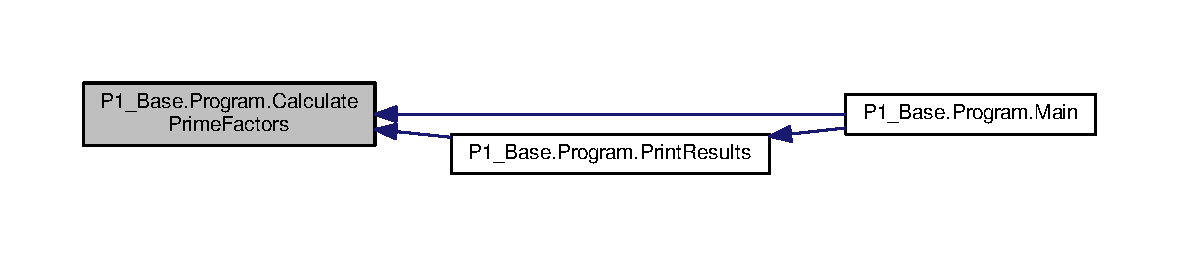
\includegraphics[width=350pt]{class_p1___base_1_1_program_a2efc0cfb173d9412a525b1657335c150_icgraph}
\end{center}
\end{figure}


\hypertarget{class_p1___base_1_1_program_a647a21fde18592bc0f35077d07d60476}{\index{P1\-\_\-\-Base\-::\-Program@{P1\-\_\-\-Base\-::\-Program}!Greatest\-Common\-Factor@{Greatest\-Common\-Factor}}
\index{Greatest\-Common\-Factor@{Greatest\-Common\-Factor}!P1_Base::Program@{P1\-\_\-\-Base\-::\-Program}}
\subsubsection[{Greatest\-Common\-Factor}]{\setlength{\rightskip}{0pt plus 5cm}static int P1\-\_\-\-Base.\-Program.\-Greatest\-Common\-Factor (
\begin{DoxyParamCaption}
\item[{int}]{a, }
\item[{int}]{b}
\end{DoxyParamCaption}
)\hspace{0.3cm}{\ttfamily [inline]}, {\ttfamily [static]}}}\label{class_p1___base_1_1_program_a647a21fde18592bc0f35077d07d60476}
Calculates the greatest commn factor of two given numbers 
\begin{DoxyParams}{Parameters}
{\em a} & the first number to be used in calculating G\-C\-F \\
\hline
{\em b} & the second number to be used in calculating G\-C\-F \\
\hline
\end{DoxyParams}
\begin{DoxyReturn}{Returns}
int\-: the greatest common factor 
\end{DoxyReturn}


Definition at line 139 of file Program.\-cs.



Here is the caller graph for this function\-:\nopagebreak
\begin{figure}[H]
\begin{center}
\leavevmode
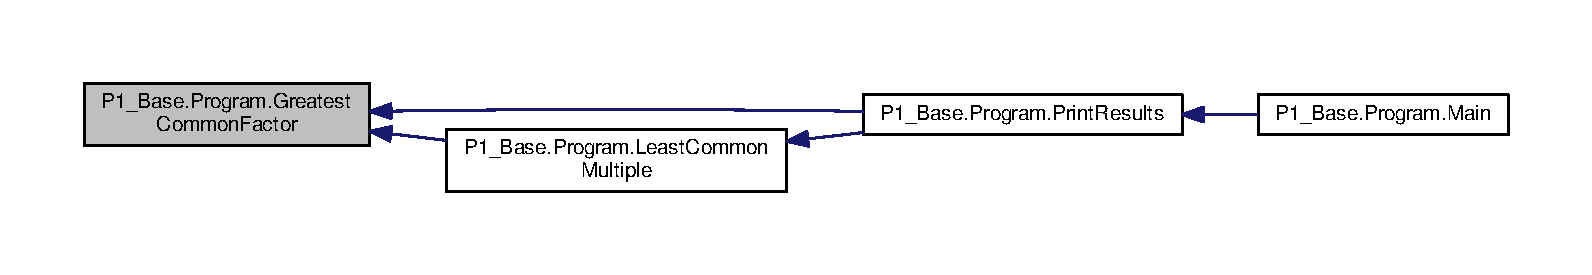
\includegraphics[width=350pt]{class_p1___base_1_1_program_a647a21fde18592bc0f35077d07d60476_icgraph}
\end{center}
\end{figure}


\hypertarget{class_p1___base_1_1_program_a771ba62e167d841cc2bb0213e5daf1a9}{\index{P1\-\_\-\-Base\-::\-Program@{P1\-\_\-\-Base\-::\-Program}!Least\-Common\-Multiple@{Least\-Common\-Multiple}}
\index{Least\-Common\-Multiple@{Least\-Common\-Multiple}!P1_Base::Program@{P1\-\_\-\-Base\-::\-Program}}
\subsubsection[{Least\-Common\-Multiple}]{\setlength{\rightskip}{0pt plus 5cm}static int P1\-\_\-\-Base.\-Program.\-Least\-Common\-Multiple (
\begin{DoxyParamCaption}
\item[{int}]{a, }
\item[{int}]{b}
\end{DoxyParamCaption}
)\hspace{0.3cm}{\ttfamily [inline]}, {\ttfamily [static]}}}\label{class_p1___base_1_1_program_a771ba62e167d841cc2bb0213e5daf1a9}
Calculates the least common multiples using $\vert$a$\ast$b$\vert$/\-G\-C\-F(a, b) 
\begin{DoxyParams}{Parameters}
{\em a} & the first number to be used in calculating L\-C\-M \\
\hline
{\em b} & the second number to be used in calculating L\-C\-M \\
\hline
\end{DoxyParams}
\begin{DoxyReturn}{Returns}
int\-: least common multiple 
\end{DoxyReturn}


Definition at line 125 of file Program.\-cs.



Here is the caller graph for this function\-:\nopagebreak
\begin{figure}[H]
\begin{center}
\leavevmode
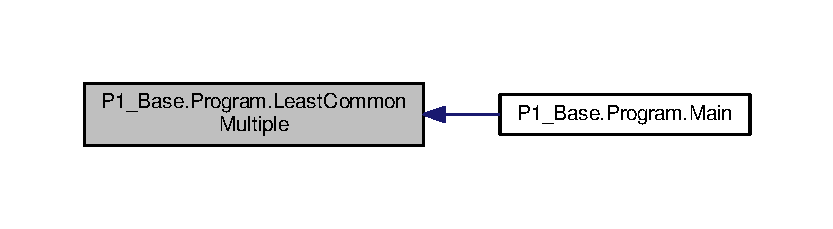
\includegraphics[width=350pt]{class_p1___base_1_1_program_a771ba62e167d841cc2bb0213e5daf1a9_icgraph}
\end{center}
\end{figure}


\hypertarget{class_p1___base_1_1_program_aacae8edf45b15eff203ad95d08a6d39b}{\index{P1\-\_\-\-Base\-::\-Program@{P1\-\_\-\-Base\-::\-Program}!Main@{Main}}
\index{Main@{Main}!P1_Base::Program@{P1\-\_\-\-Base\-::\-Program}}
\subsubsection[{Main}]{\setlength{\rightskip}{0pt plus 5cm}static void P1\-\_\-\-Base.\-Program.\-Main (
\begin{DoxyParamCaption}
\item[{string\mbox{[}$\,$\mbox{]}}]{args}
\end{DoxyParamCaption}
)\hspace{0.3cm}{\ttfamily [inline]}, {\ttfamily [static]}, {\ttfamily [private]}}}\label{class_p1___base_1_1_program_aacae8edf45b15eff203ad95d08a6d39b}
Driver method 

Definition at line 22 of file Program.\-cs.



Here is the call graph for this function\-:\nopagebreak
\begin{figure}[H]
\begin{center}
\leavevmode
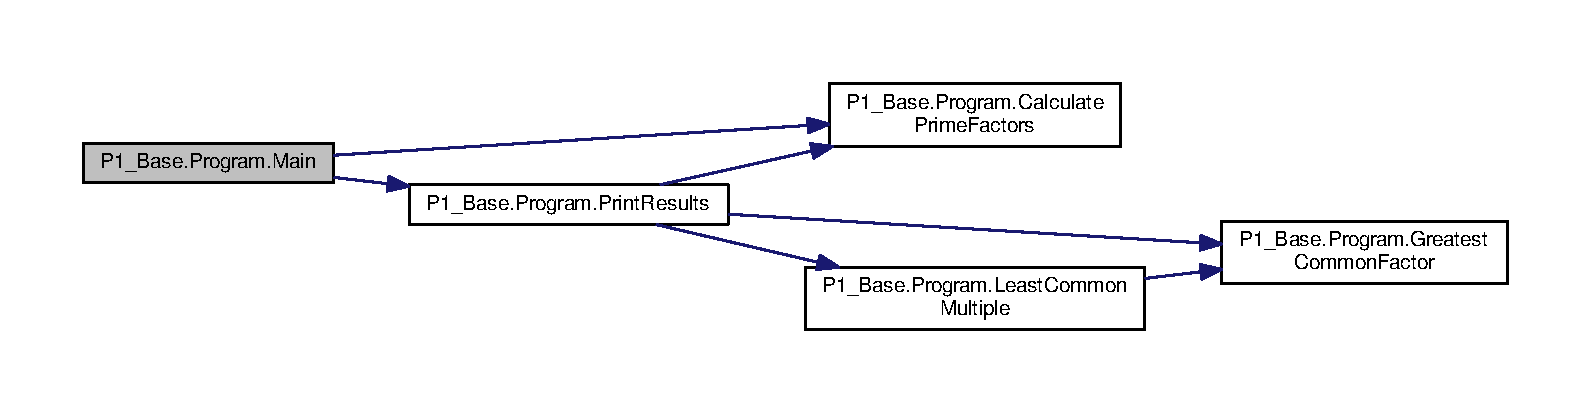
\includegraphics[width=350pt]{class_p1___base_1_1_program_aacae8edf45b15eff203ad95d08a6d39b_cgraph}
\end{center}
\end{figure}




\subsection{Field Documentation}
\hypertarget{class_p1___base_1_1_program_a5a1d1aaa0c9be4b481faddab1e1ab753}{\index{P1\-\_\-\-Base\-::\-Program@{P1\-\_\-\-Base\-::\-Program}!prime\-Factor\-A@{prime\-Factor\-A}}
\index{prime\-Factor\-A@{prime\-Factor\-A}!P1_Base::Program@{P1\-\_\-\-Base\-::\-Program}}
\subsubsection[{prime\-Factor\-A}]{\setlength{\rightskip}{0pt plus 5cm}List$<$int$>$ P1\-\_\-\-Base.\-Program.\-prime\-Factor\-A = new List$<$int$>$()\hspace{0.3cm}{\ttfamily [static]}, {\ttfamily [private]}}}\label{class_p1___base_1_1_program_a5a1d1aaa0c9be4b481faddab1e1ab753}
Holds the prime factors of the first number passed 

Definition at line 14 of file Program.\-cs.

\hypertarget{class_p1___base_1_1_program_ab76652179b4151a50e1fadf328abdb44}{\index{P1\-\_\-\-Base\-::\-Program@{P1\-\_\-\-Base\-::\-Program}!prime\-Factor\-B@{prime\-Factor\-B}}
\index{prime\-Factor\-B@{prime\-Factor\-B}!P1_Base::Program@{P1\-\_\-\-Base\-::\-Program}}
\subsubsection[{prime\-Factor\-B}]{\setlength{\rightskip}{0pt plus 5cm}List$<$int$>$ P1\-\_\-\-Base.\-Program.\-prime\-Factor\-B = new List$<$int$>$()\hspace{0.3cm}{\ttfamily [static]}, {\ttfamily [private]}}}\label{class_p1___base_1_1_program_ab76652179b4151a50e1fadf328abdb44}
Holds the prime factores of the second number passed 

Definition at line 18 of file Program.\-cs.



The documentation for this class was generated from the following file\-:\begin{DoxyCompactItemize}
\item 
\hyperlink{_program_8cs}{Program.\-cs}\end{DoxyCompactItemize}

\chapter{File Documentation}
\hypertarget{_debug_2_p1___base_8csproj_8_file_list_absolute_8txt}{\section{obj/\-Debug/\-P1\-\_\-\-Base.csproj.\-File\-List\-Absolute.\-txt File Reference}
\label{_debug_2_p1___base_8csproj_8_file_list_absolute_8txt}\index{obj/\-Debug/\-P1\-\_\-\-Base.\-csproj.\-File\-List\-Absolute.\-txt@{obj/\-Debug/\-P1\-\_\-\-Base.\-csproj.\-File\-List\-Absolute.\-txt}}
}

\hypertarget{_release_2_p1___base_8csproj_8_file_list_absolute_8txt}{\section{obj/\-Release/\-P1\-\_\-\-Base.csproj.\-File\-List\-Absolute.\-txt File Reference}
\label{_release_2_p1___base_8csproj_8_file_list_absolute_8txt}\index{obj/\-Release/\-P1\-\_\-\-Base.\-csproj.\-File\-List\-Absolute.\-txt@{obj/\-Release/\-P1\-\_\-\-Base.\-csproj.\-File\-List\-Absolute.\-txt}}
}

\hypertarget{_temporary_generated_file__036_c0_b5_b-1481-4323-8_d20-8_f5_a_d_c_b23_d92_8cs}{\section{obj/\-Debug/\-Temporary\-Generated\-File\-\_\-036\-C0\-B5\-B-\/1481-\/4323-\/8\-D20-\/8\-F5\-A\-D\-C\-B23\-D92.cs File Reference}
\label{_temporary_generated_file__036_c0_b5_b-1481-4323-8_d20-8_f5_a_d_c_b23_d92_8cs}\index{obj/\-Debug/\-Temporary\-Generated\-File\-\_\-036\-C0\-B5\-B-\/1481-\/4323-\/8\-D20-\/8\-F5\-A\-D\-C\-B23\-D92.\-cs@{obj/\-Debug/\-Temporary\-Generated\-File\-\_\-036\-C0\-B5\-B-\/1481-\/4323-\/8\-D20-\/8\-F5\-A\-D\-C\-B23\-D92.\-cs}}
}

\hypertarget{_temporary_generated_file__5937a670-0e60-4077-877b-f7221da3dda1_8cs}{\section{obj/\-Debug/\-Temporary\-Generated\-File\-\_\-5937a670-\/0e60-\/4077-\/877b-\/f7221da3dda1.cs File Reference}
\label{_temporary_generated_file__5937a670-0e60-4077-877b-f7221da3dda1_8cs}\index{obj/\-Debug/\-Temporary\-Generated\-File\-\_\-5937a670-\/0e60-\/4077-\/877b-\/f7221da3dda1.\-cs@{obj/\-Debug/\-Temporary\-Generated\-File\-\_\-5937a670-\/0e60-\/4077-\/877b-\/f7221da3dda1.\-cs}}
}

\hypertarget{_temporary_generated_file___e7_a71_f73-0_f8_d-4_b9_b-_b56_e-8_e70_b10_b_c5_d3_8cs}{\section{obj/\-Debug/\-Temporary\-Generated\-File\-\_\-\-E7\-A71\-F73-\/0\-F8\-D-\/4\-B9\-B-\/\-B56\-E-\/8\-E70\-B10\-B\-C5\-D3.cs File Reference}
\label{_temporary_generated_file___e7_a71_f73-0_f8_d-4_b9_b-_b56_e-8_e70_b10_b_c5_d3_8cs}\index{obj/\-Debug/\-Temporary\-Generated\-File\-\_\-\-E7\-A71\-F73-\/0\-F8\-D-\/4\-B9\-B-\/\-B56\-E-\/8\-E70\-B10\-B\-C5\-D3.\-cs@{obj/\-Debug/\-Temporary\-Generated\-File\-\_\-\-E7\-A71\-F73-\/0\-F8\-D-\/4\-B9\-B-\/\-B56\-E-\/8\-E70\-B10\-B\-C5\-D3.\-cs}}
}

\hypertarget{_program_8cs}{\section{Program.\-cs File Reference}
\label{_program_8cs}\index{Program.\-cs@{Program.\-cs}}
}
\subsection*{Data Structures}
\begin{DoxyCompactItemize}
\item 
class \hyperlink{class_p1___base_1_1_program}{P1\-\_\-\-Base.\-Program}
\end{DoxyCompactItemize}
\subsection*{Namespaces}
\begin{DoxyCompactItemize}
\item 
package \hyperlink{namespace_p1___base}{P1\-\_\-\-Base}
\end{DoxyCompactItemize}

\hypertarget{_assembly_info_8cs}{\section{Properties/\-Assembly\-Info.cs File Reference}
\label{_assembly_info_8cs}\index{Properties/\-Assembly\-Info.\-cs@{Properties/\-Assembly\-Info.\-cs}}
}

\hypertarget{_r_e_a_d_m_e_8md}{\section{R\-E\-A\-D\-M\-E.\-md File Reference}
\label{_r_e_a_d_m_e_8md}\index{R\-E\-A\-D\-M\-E.\-md@{R\-E\-A\-D\-M\-E.\-md}}
}

%--- End generated contents ---

% Index
\newpage
\phantomsection
\addcontentsline{toc}{chapter}{Index}
\printindex

\end{document}
